\documentclass[../main/main.tex]{subfiles}

\newdate{date}{08}{10}{2020}


\begin{document}

\marginpar{ \textbf{Lecture 3.} \\  \displaydate{date}. \\ Compiled:  \today.}

\section{Basic models}

We are gonna introduce some of the basic models we will deal for the entire course.
We are assuming that we are in \textbf{well-mixed populations}, or homogeneous mixing. Mathematically, it is what is called mean field approximation.
In the well-mixed population assumptions, we are assuming that:
\begin{itemize}
\item all individuals are equivalent, hence every one has the same probability of getting the infection;
\item every individual has the same number of contacts \( N-1 \), or on average \( \expval{k}  \);
\item another important assumption is that we are in a closed population. Hence, the sum of the density distribution of the individuals is 1 and we have no deaths or births. In practice, we are assuming that our time scale is so little that we can consider the population constant.
\end{itemize}

\subsection{SI model}

This simple model is the \textbf{SI} (susceptible infected). You can get the infection and once you get it you cannot recover (you stay infected forever).
The transition is:
\begin{equation}
  S + I \overset{\beta }{\rightarrow} I + I
\end{equation}
The \( \beta  \) is the “per contact” infection rate and dictates the speed of the spreading. We can write down the equation and solve it deterministically:
\begin{equation}
\begin{split}
  \dv{s}{t} &= - \beta \expval{k} s i \\ \dv{i}{t} &= \beta \expval{k} s i
\end{split}
\end{equation}
where \( \expval{k}  \) represents the contacts, the \( i \) means the fraction of infected in the population (\( i=I/N \)), while \( s \) the fraction of susceptible in the population (\( s=S/N \)).
The product \( s i \) is the probability of contacts, and \( \beta  s i \) is the proabability of having one more infected.

To solve it analitically, we should remember that our population is closed hence \( s+i=1 \), we only have one equation with \( s=1-i \).
We have that:
\begin{equation*}
  \dv{i}{t} = \beta i (1-i) \quad \rightarrow \frac{1}{\beta i (1-i)} \dd[]{i} = \dd[]{t} \quad \rightarrow \frac{1}{\beta (1-i)} \dd[]{i} + \frac{1}{\beta i} \dd[]{i} = \dd[]{t}
\end{equation*}
Integrating both sides:
\begin{equation*}
  - \log \abs{1-i} + \log \abs{i} = \beta (t+C) \rightarrow \frac{i}{1-i} = e^{\beta (t+C)} = A e^{\beta t}
\end{equation*}
with \( A = i_0/(1-i_0) \).
% See the calculus in Fig. \ref{fig:3_1}.
% \begin{figure}[h!]
% \centering
% 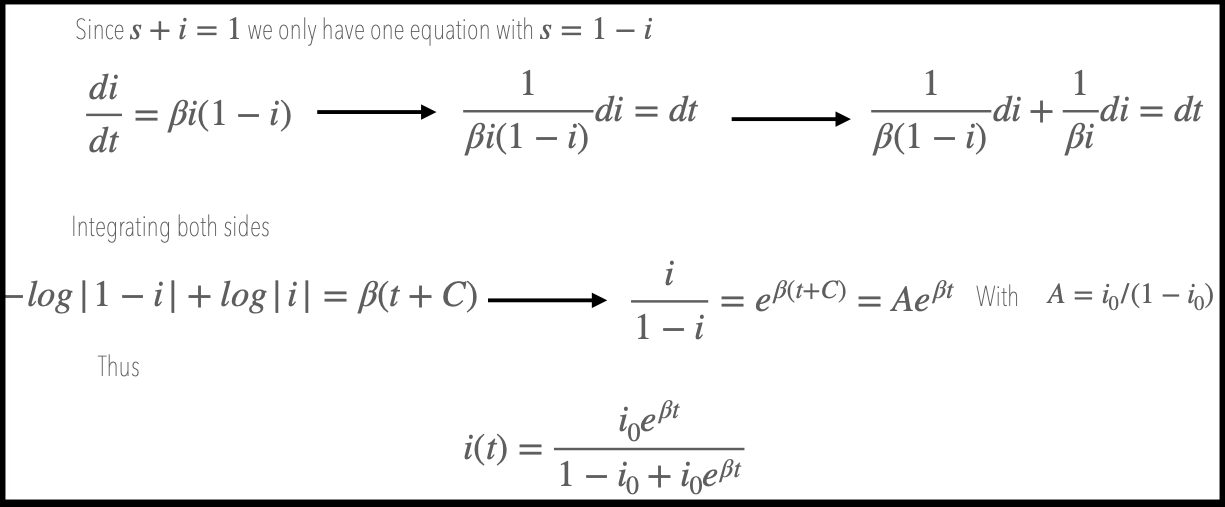
\includegraphics[width=0.9\textwidth]{../lessons/image/03/1.png}
% \caption{\label{fig:3_1} Calculation of the analitic solution for the SI model.}
% \end{figure}
The result is:
\begin{equation}
  i(t) = \frac{i_0 e^{\beta t} }{1-i_0 + i_0 e^{\beta t} }
\end{equation}
which is a sigmoid function (Fig. \ref{fig:3_2}) which always saturates at 1. We have the first part where we have the exponential growth (which is the one we have seen in the media for covid-19), then at a certain point you are slowing down. The reason of slowing down is because of the term \( s i \), the probability of funding new supsceptible is going down. Finally, you reach 1 after a very long time. The value of \( \beta  \) is the one which drives the spreading. Increasing \( \beta  \) we have a faster exponential growth.
This was the simplest model.

\begin{figure}[h!]
\centering
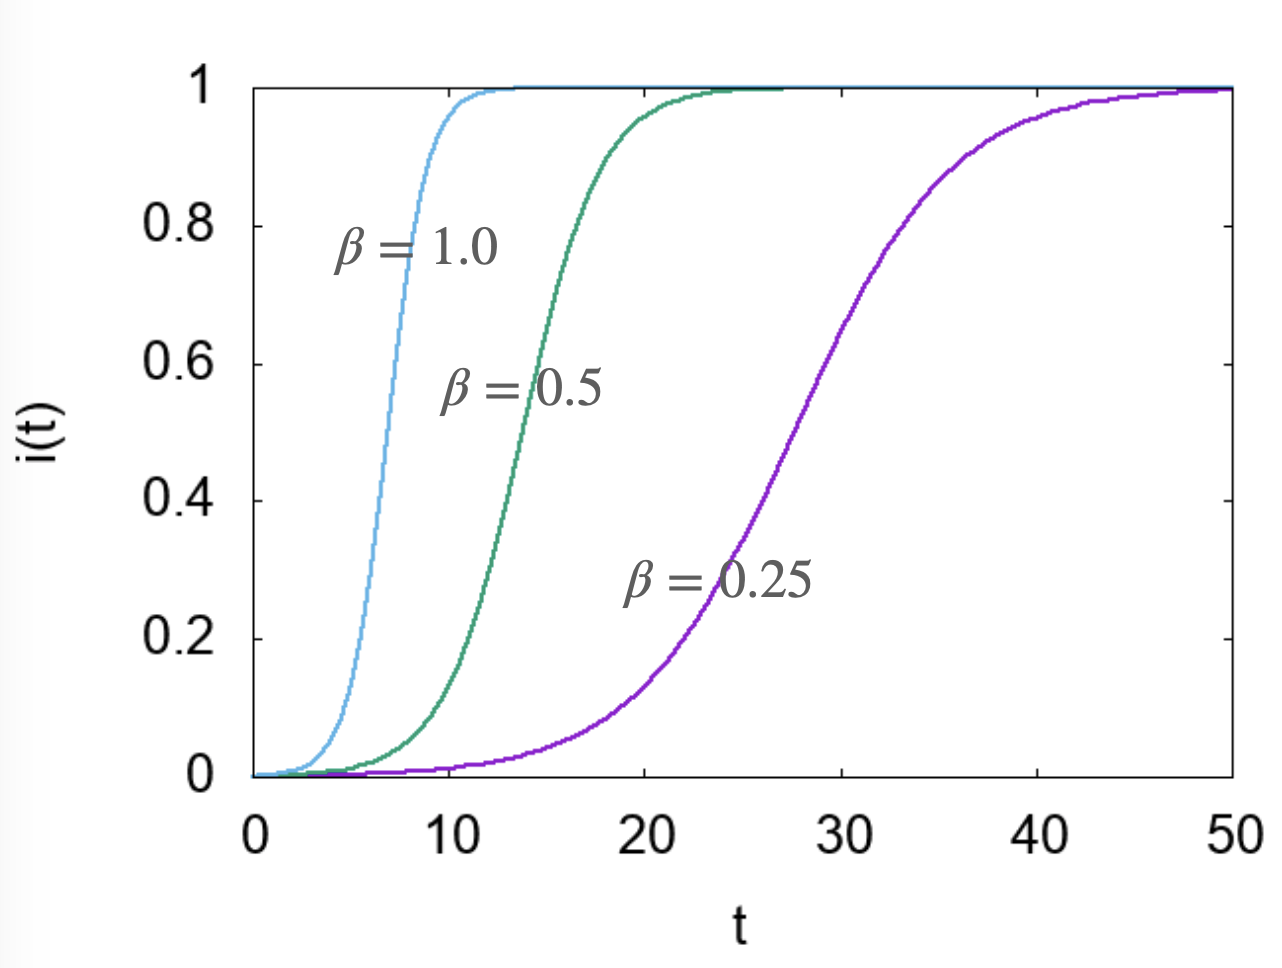
\includegraphics[width=0.7\textwidth]{../lessons/image/03/2.png}
\caption{\label{fig:3_2} Plot of the solution of the SI model for different \( \beta  \).}
\end{figure}

\begin{remark}
In the course we are gonna use capital letter for integer numbers and small lecter for densities.
\end{remark}

\subsection{SIS model}
Now, let us go to the \textbf{SIS} model. This model starts to be more complicated. We have two different transitions:
\begin{equation}
\begin{split}
  S + I &\overset{\beta }{\rightarrow } I + I \\
  I &\overset{\mu }{\rightarrow } S
\end{split}
\end{equation}
whose second one is spontaneous.
This model is used for diseases that do not confer immunity. \textbf{Endemic state} means that the disease circulates in the population for very large times.
The important things is that it is the simplest models in which a dynamical equilibrium can be reached. An individual could recover after the disease but it do not get immunity, indeed there are always people infected that can propagate the disease. The \( \mu  \) is the recovery rate which determines the time-scale of the infection.
Dividing \( \beta  \) by \( \mu  \) you can rescale all the dynamics.
The equations are exactly the same of before except for a term:
\begin{equation}
\begin{split}
  \dv{s}{t} &= - \beta \expval{k} si + \mathcolorbox{green!20}{\mu i}  \\
  \dv{i}{t} &= \beta \expval{k} si - \mathcolorbox{green!20}{\mu i}
\end{split}
\end{equation}
and you can solve them in the way of before.
Also the shape of the solution is exactly the same:
\begin{equation}
  i(t) = i_0 \frac{(\beta - \mu ) e^{(\beta - \mu )t} }{\beta - \mu  + \beta i_0 e^{(\beta - \mu )t} }
\end{equation}
If we plot it we have the same form but with the difference that we are not reaching one, but \( \frac{\beta - \mu }{\beta } \). Hence, as said, we have some sort of dynamical equilibrium: the new infected are the same of the new recovery that you are getting. The population will fluctuate around this value \( \frac{\beta - \mu }{\beta } \) and enlarging \( \mu  \) will give to larging fluctuations (Fig. \ref{fig:3_3}).
\begin{figure}[h!]
\centering
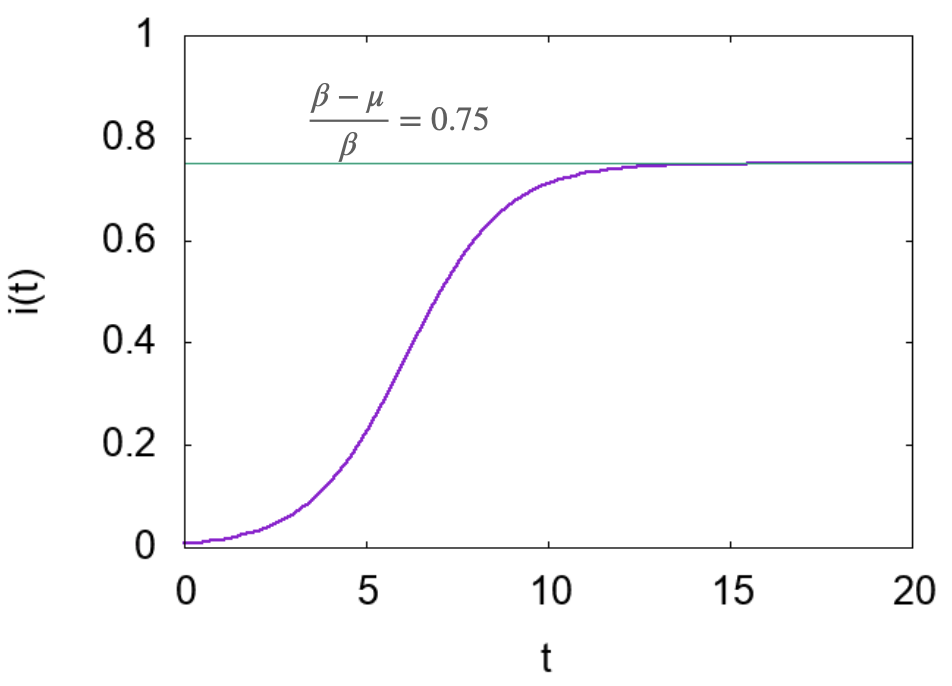
\includegraphics[width=0.7\textwidth]{../lessons/image/03/3.png}
\caption{\label{fig:3_3} Plot of the solution of the SIS model.}
\end{figure}

It could be more instructive to study what happens at the beginning for this model. At the beginning I can assume that almost my population is composed by my susceptible (\( s \sim 1 \)) and the number of infected is very little (\( i \ll 1 \)).
Hence, we can rewrite the differential equations as:
\begin{equation*}
  \dv{i}{t} = \beta \expval{k} s i - \mu i \sim \beta \expval{k} i - \mu i \rightarrow i(t) \sim i_0 e^{(\beta \expval{k} - \mu  )t}
\end{equation*}
We have that if \( \beta \expval{k} < \mu   \) I have not spreading at this point, while if \( \beta \expval{k} > \mu   \) the exponential becomes positive and I have the exponential growing at the beginning (Fig. \ref{fig:3_4}).

\begin{figure}[h!]
\centering
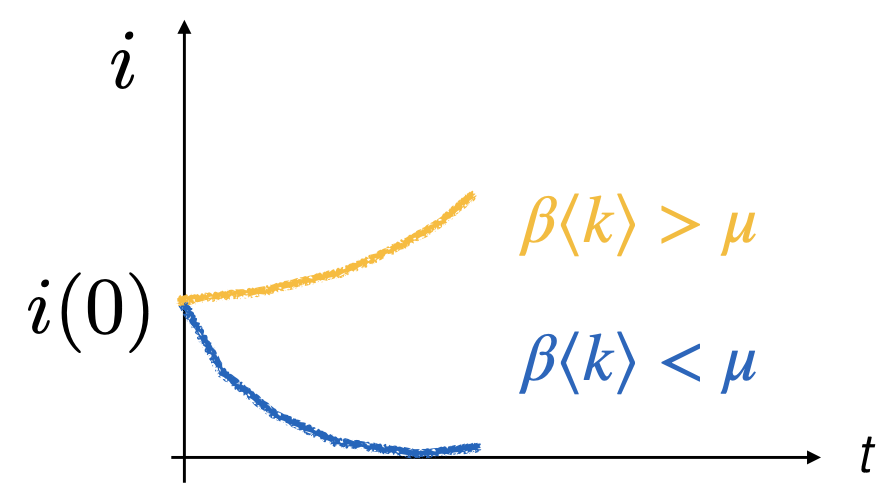
\includegraphics[width=0.6\textwidth]{../lessons/image/03/4.png}
\caption{\label{fig:3_4} Initial transient for the SIS model.}
\end{figure}

The very important thing is that if I consider what it is happening I have two choices for the steady state:
\begin{equation*}
  \dv{i}{t} = 0 \rightarrow  \begin{cases}
   i=0 & \beta \expval{k} < \mu  \\
   i>0 & \beta \expval{k} > \mu
  \end{cases}
\end{equation*}
and we have that:
\begin{equation}
  i>0 \iff \beta > \beta_c = \frac{\mu }{ \expval{k} }
\end{equation}
which is the \textbf{epidemic threshold}. This is telling you if the disease is gonne spread.
The epidemic threshold is the minimum value of the infection probability for which the disease survives. This is what in physics is called a second order phase transition (Fig. \ref{fig:3_5}). In this case the critical exponents are the same of the Ising model (they are in the same class of universality).
This is one of the most important quantities we are gonna study.

\begin{figure}[h!]
\centering
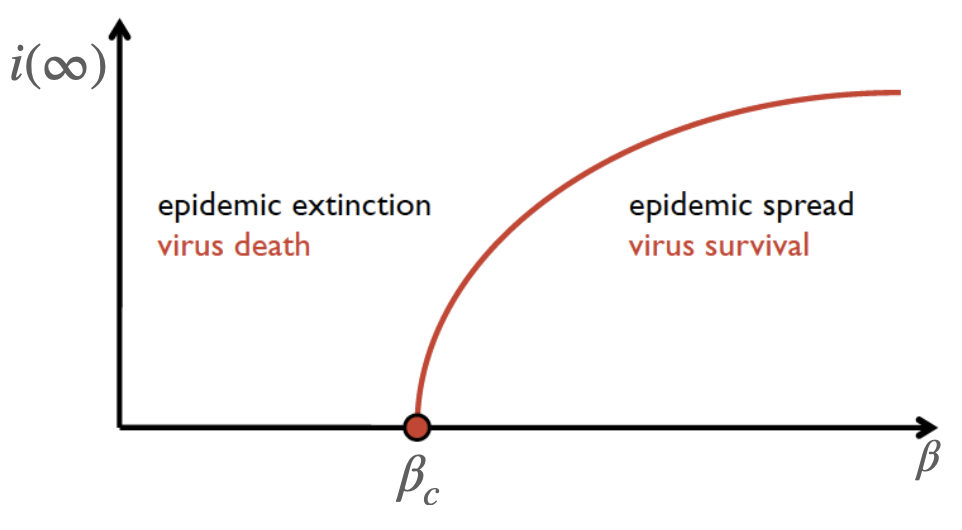
\includegraphics[width=0.7\textwidth]{../lessons/image/03/5.png}
\caption{\label{fig:3_5} Epidemic diagram.}
\end{figure}

What is the relation between \( R_0 \) and the epidemic threshold? Obviously, they are strongly correlated. We are saying that we have a critical value and below it we have no spreading, while above we have a fraction of infected people.
The epidemic threshold is given you the condition under which you have the spreading. Mathematically, giving a speficic model, its critical version is giving the value for which \( R_0=1 \), which means that if you are above the threshold you need a minimum of infected people which is 1.  In the case of the SIS model:
\begin{equation}
  R_0 = \frac{\beta \expval{k} }{\mu } = 1
\end{equation}


\subsection{SIR model}
The idea is the same of the SIS, but we are adding a new state which accounts for long lasting immunity. Hence, once you got the disease you can have a long immunity. However, the density of the population is still fixed to 1. The transitions of this model are:
\begin{equation}
\begin{split}
  S + I &\overset{\beta }{\rightarrow } I + I  \\
  I &\overset{\mu }{\rightarrow } R
\end{split}
\end{equation}
and we have no endemic state.
The differential equations are:
\begin{equation}
\begin{split}
  \dv{s}{t} &= - \beta \expval{k} si  \\
  \dv{i}{t} &= \overbrace{\beta \expval{k} si}^{\text{New infections}}  - \overbrace{\mu i}^{\text{Recovery}} \\
  \dv{r}{t} &= \mu i
\end{split}
\end{equation}

\begin{figure}[h!]
\centering
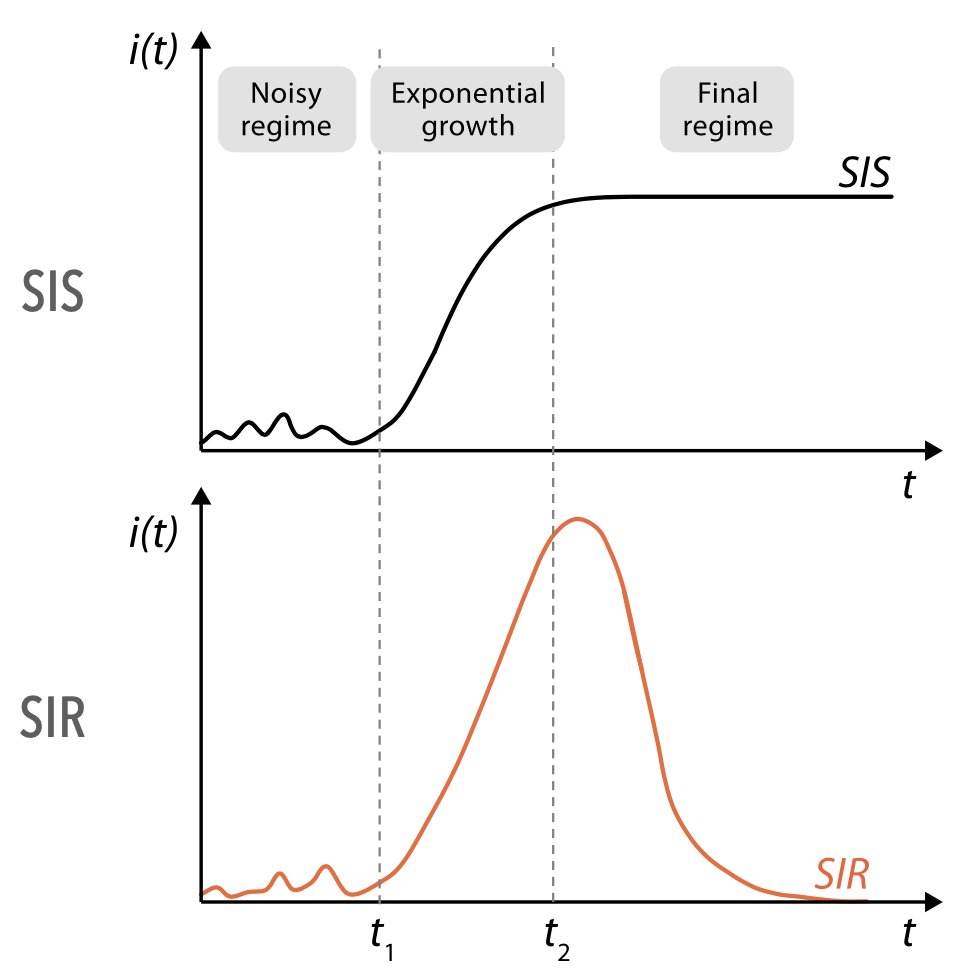
\includegraphics[width=0.6\textwidth]{../lessons/image/03/6.png}
\caption{\label{fig:3_6} Epidemic regimes.}
\end{figure}

It is a good point to introduce the different regimes that you have during a spreading and which are represented in Fig. \ref{fig:3_6} for the  SIS and SIR models.
Initially, at the beginning of each spreading, you have the \textbf{noisy phases} where the numbers are too small to cause a spreading, hence you have a sort of stocastic fluctuations. In most of the cases, you can end up without infected. If you stop a guy in this noisy phase, you are able to stop the disease (if it is hetherogeneous). Then, we have the \textbf{exponential growth}. Then, the disease is slowing down. Finally, you reach the steady state for the SIS (endemic state), while for the SIR the disease disappear (absorbing state).

To calculate the epidemic threshold in the case of the SIR the calculations are the same of before. In particular, we assume that \( r \ll 1 \) so that:
\begin{equation*}
  \dv{i}{t} = \beta \expval{k} s i - \mu i \sim \beta \expval{k} i - \mu i \rightarrow i(t) \sim i_0 e^{(\beta \expval{k} - \mu  )t}
\end{equation*}
and the result is again:
\begin{equation}
  \beta > \beta _c = \frac{\mu }{\expval{k} }
\end{equation}

Since we can get an analitic expression for S and I in this SIR model, we want to study what is the behavior at the end for \( t = \infty  \). We get that:
\begin{equation*}
  \dv{s}{r} = \frac{- \beta  \expval{k}  s}{\mu }
\end{equation*}
If we assume \( r_0 = 0  \) and we integrate the above expression with respect to \( r \), we obtain:
\begin{equation*}
  s(t) = s_0 e^{-r(t) \frac{\beta \expval{k} }{\mu }}
\end{equation*}
As said, we cannot solve this equation directly, but we can study the behavior in the long term. At \( t=\infty  \), we have that \( i (\infty ) = 0 \) and thus \( s(\infty ) = 1 - r(\infty ) \):
\begin{equation*}
  1 - r(\infty ) - s_0 e^{-r(\infty ) \overbrace{\frac{\beta \expval{k} }{\mu }}^{R_0}} = 0
\end{equation*}
This is a transcendental equation which cannot be solved analytically but it gives important hints on the behavior of the disease.
Note that \( R_0 = \beta \expval{k} / \mu   \) and this explains why \( R_0 \) drives the exponential growth of the disease. Moreover, we note that the initial fraction \( s_0 \) of susceptible plays a role in shaping the final fraction of recovered.
In particular, if \( s_0 \ll 1 \) the disease cannot spread. We can obtain herd immunity.




\section{Extensions of the SIR model}
We want to modify the SIR to include something that we want in our model.

\subsection{SIR with Demography}
In the last models, we were assuming that the population was totally closed and so it always sum up to 1. This is one thing that we want to remove because it is unrealistic. We will assume that there could be births and deaths.
If we consider the demography, we see that every year there are new child that are infected by disease as Measles and Chickenpox. We expect that usually they die out over weeks.

Hence, the simplest assumption is: similar to the infectious period, individuals have a lifespan \( 1/\alpha  \) years (where lifespan is much greater than the infectious period, deaths are not due to the disease).
We are assuming that \( \alpha  \) is the death rate in all the classes. Moreover, \( \alpha  \) is also the crude birth rate and we assume that births happens only in suscpetible individuals.

To have a constant population, we need to assume:
\begin{equation}
  \dv{s}{t} + \dv{i}{t} + \dv{r}{t} = 0
\end{equation}

Our equations become:
\begin{equation}
\begin{split}
  \dv{s}{t} &= \alpha - \beta s i - \alpha s  \\
  \dv{i}{t} &= \beta s i - \mu i - \alpha i \\
  \dv{r}{t} &= \mu i - \alpha r
\end{split}
\end{equation}
The infectious period is:
\begin{equation}
  \tau = \frac{1}{\alpha + \mu }
\end{equation}
on average, individuals spend less infected because some of them die while infected. However, it is a small change since lifespan is much greater than the infectious period.

Also \( R_0 \) is reduced due to mortality:
\begin{equation}
  R_0 = \frac{\beta }{\alpha + \mu }
\end{equation}


We want to study the equilibrium points of the dynamic. Assuming:
\begin{equation*}
  \dv{s}{t} = \dv{i}{t} = \dv{r}{t} = 0
\end{equation*}
we want to find the equilibrium values  \( s^* \), \( i^* \) and \( r^* \).
We have that:
\begin{equation*}
  \dv{i}{t} = 0 = \beta s i - \mu i - \alpha i \quad \rightarrow   \beta s^* i^* - (\mu + \alpha ) i^* = 0
\end{equation*}
and finally we obtain the equation:
\begin{equation}
  i^* \qty[\beta s^* - (\mu + \alpha )] = 0
\end{equation}
which is not differential anymore.
The two solutions are \( i^* = 0 \) (\textbf{disease free state}) or \( s^* = \frac{\alpha + \mu }{\beta } = \frac{1}{R_0} \) which is the \textbf{endemic state}. Hence, the important result is that the SIR model with demography shows an endemic state.

Substituting \( s^* = \frac{1}{R_0} \) in \( \dv{s}{t} = \alpha - \beta s i - \alpha w  \), we get:
\begin{equation*}
  i^* = \frac{\alpha }{\mu } \qty(1 - \frac{1}{R_0}) = \frac{\alpha }{\beta } (R_0 -1)
\end{equation*}
Finally, the three values of the fraction of infected, suscpetible and recovered in the endemic state are:
\begin{equation}
  (s^*, i^*, r^*) = \qty( \frac{1}{R_0}, \frac{\alpha }{\beta } (R_0 -1 ), 1- \frac{1}{R_0} - \frac{\alpha }{\beta } (R_0-1))
\end{equation}
This exists only if \( R_0>1 \). Moreover, via linear stability analysis it can be demonstrated that this equilibrium is stable and is reached through damped oscillations


\end{document}
